\section{Experimental Evaluation} \label{sec:experimental-evaluation}
This section describes the main test cases used to evaluate the solver.

\subsection{Case 1: Task 1 Movement with Different Goal Floors} \label{subsec:case-1:-task-1-movement-with-different-goal-floors}

For the movement-only task, three movers start on floor $0$:
\[
    \texttt{atFloor(Alice,0,0)}, \quad
    \texttt{atFloor(Bob,0,0)}, \quad
    \texttt{atFloor(Eve,0,0)}.
\]

\noindent In the tested configuration, the building has seven floors and the target floors are:
\[
    \texttt{Alice}@6, \qquad \texttt{Bob}@4, \qquad \texttt{Eve}@2.
\]

\noindent The solver finds an optimal plan in six steps.
This is expected because Alice must ascend from floor $0$ to floor $6$, which requires six upward movements.
Bob and Eve reach their target floors earlier and then remain idle while Alice completes the longest path.

\begin{figure}[H]
    \centering
    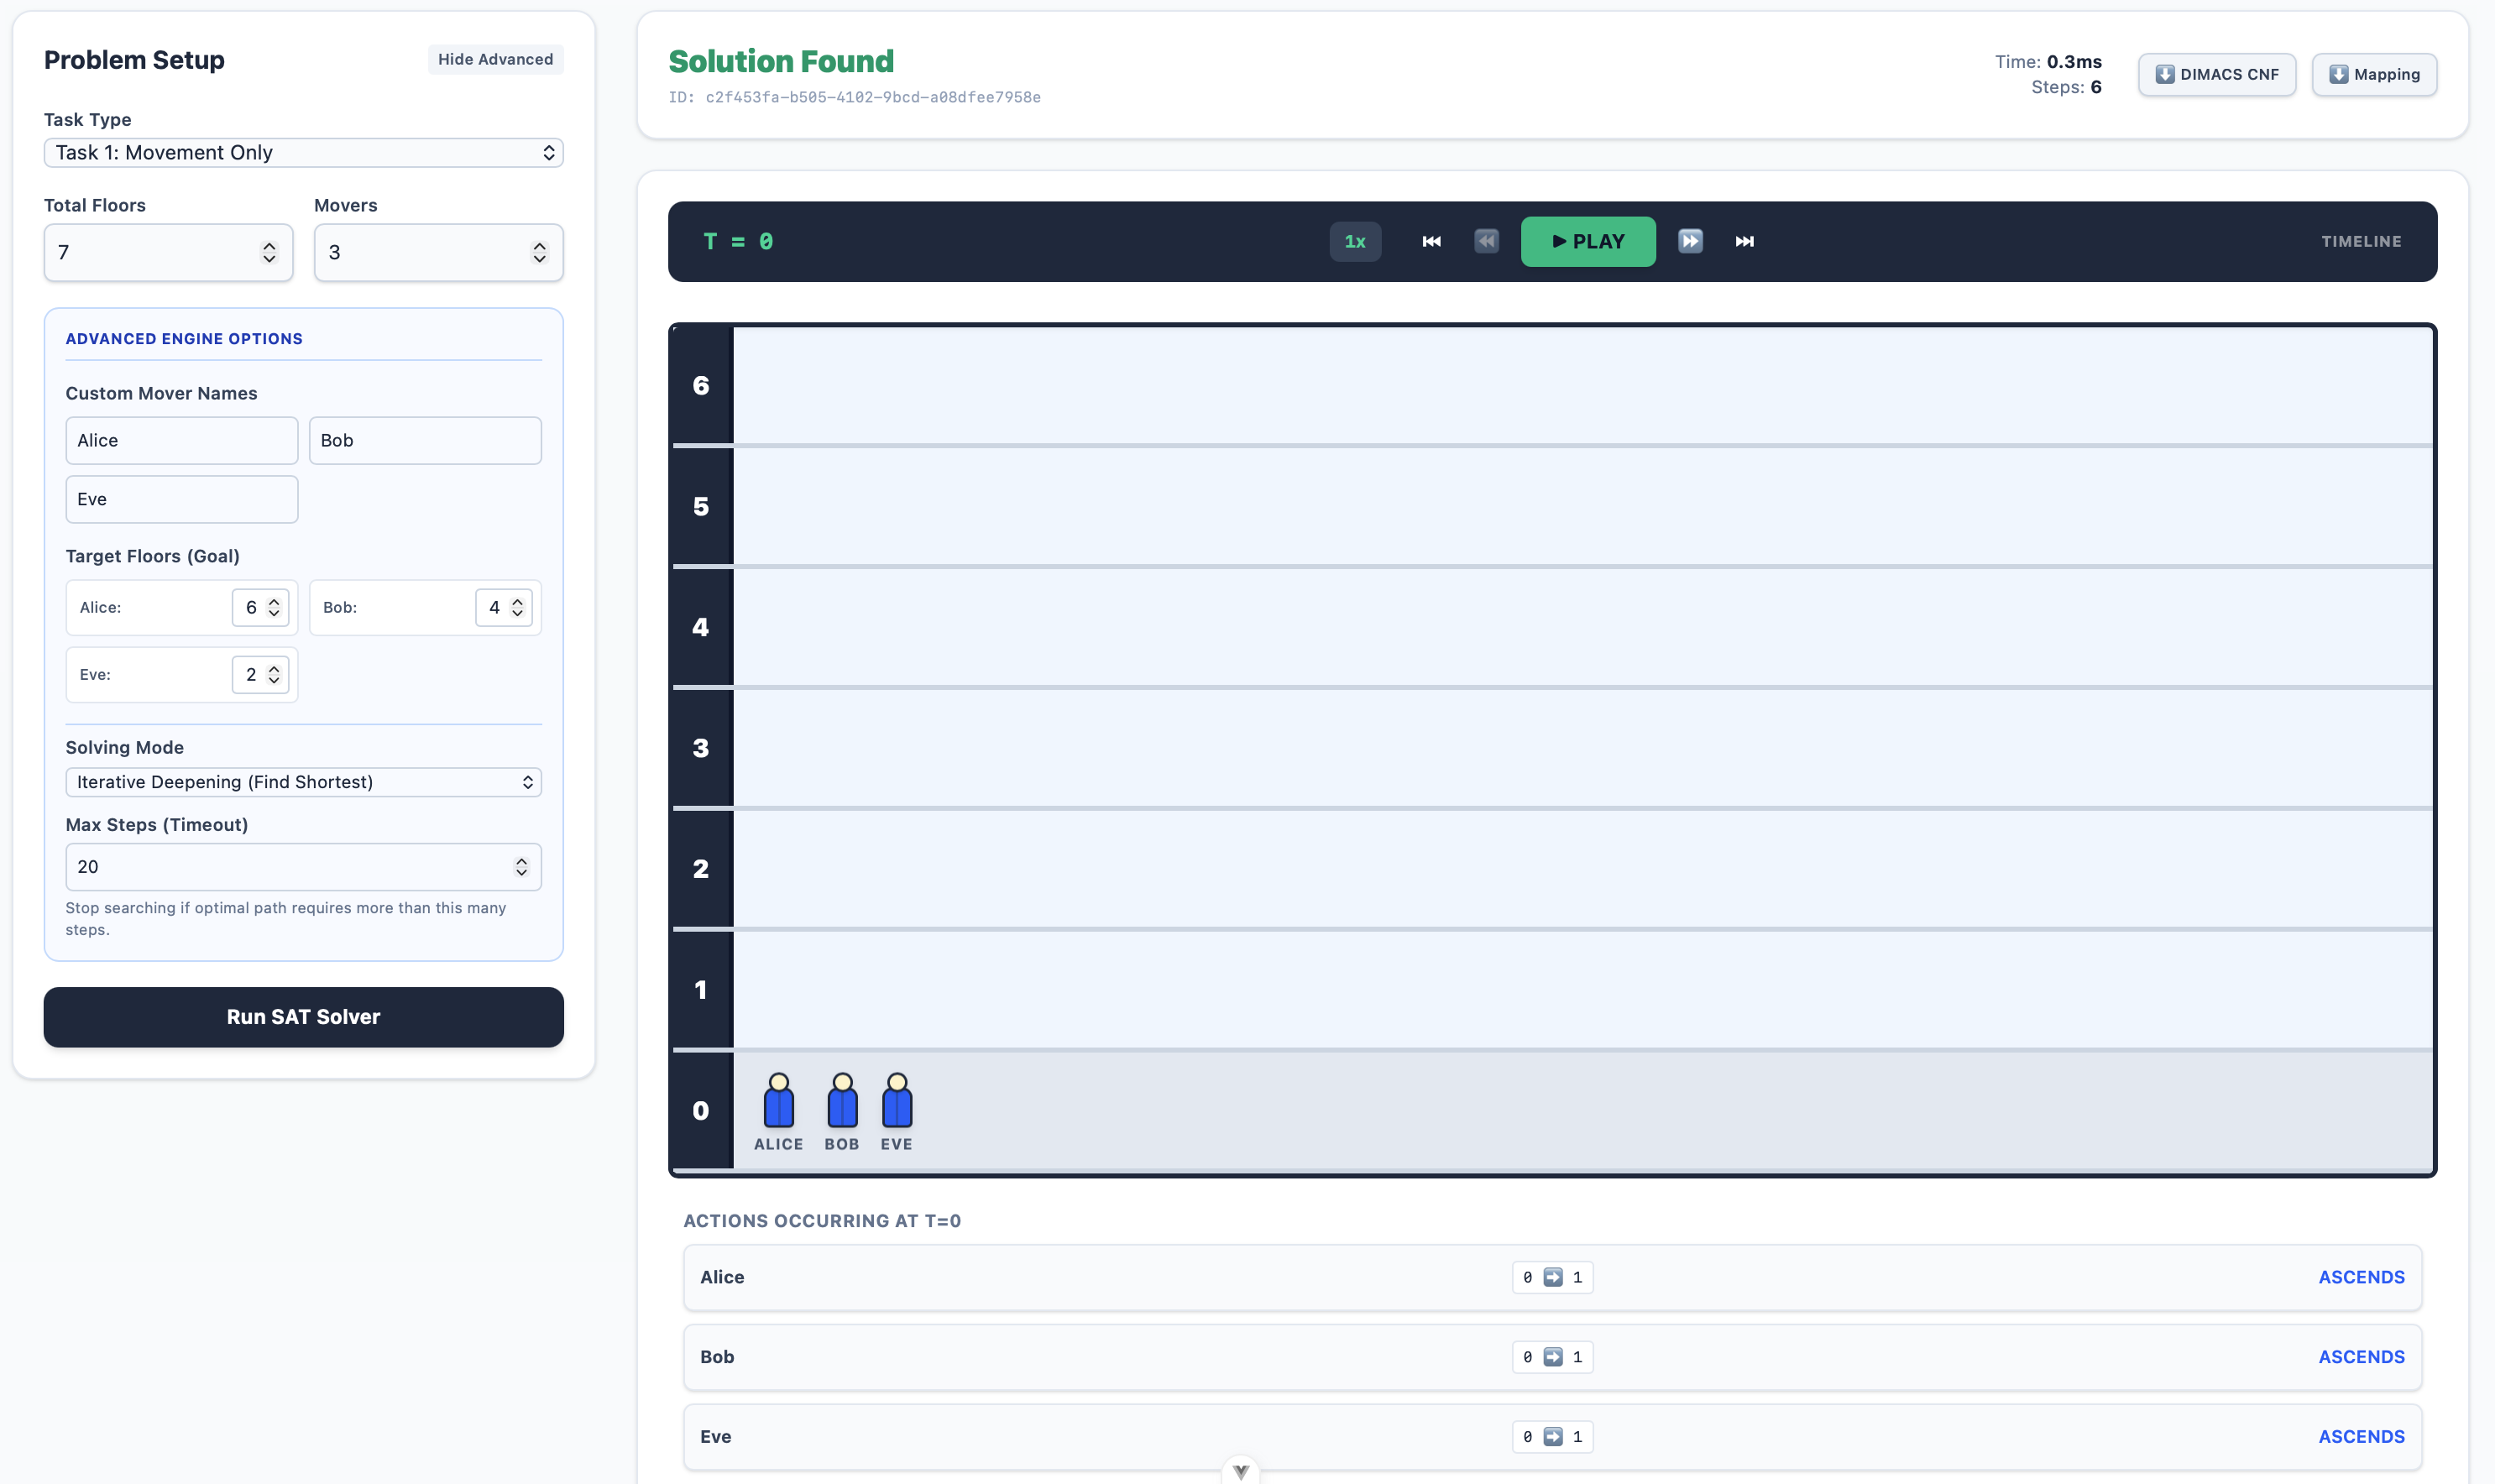
\includegraphics[width=0.95\textwidth]{img/task1-initial-state}
    \caption{Initial state of a Task 1 instance: all movers start on the ground floor.}
    \label{fig:task1-initial}
\end{figure}

\begin{figure}[H]
    \centering
    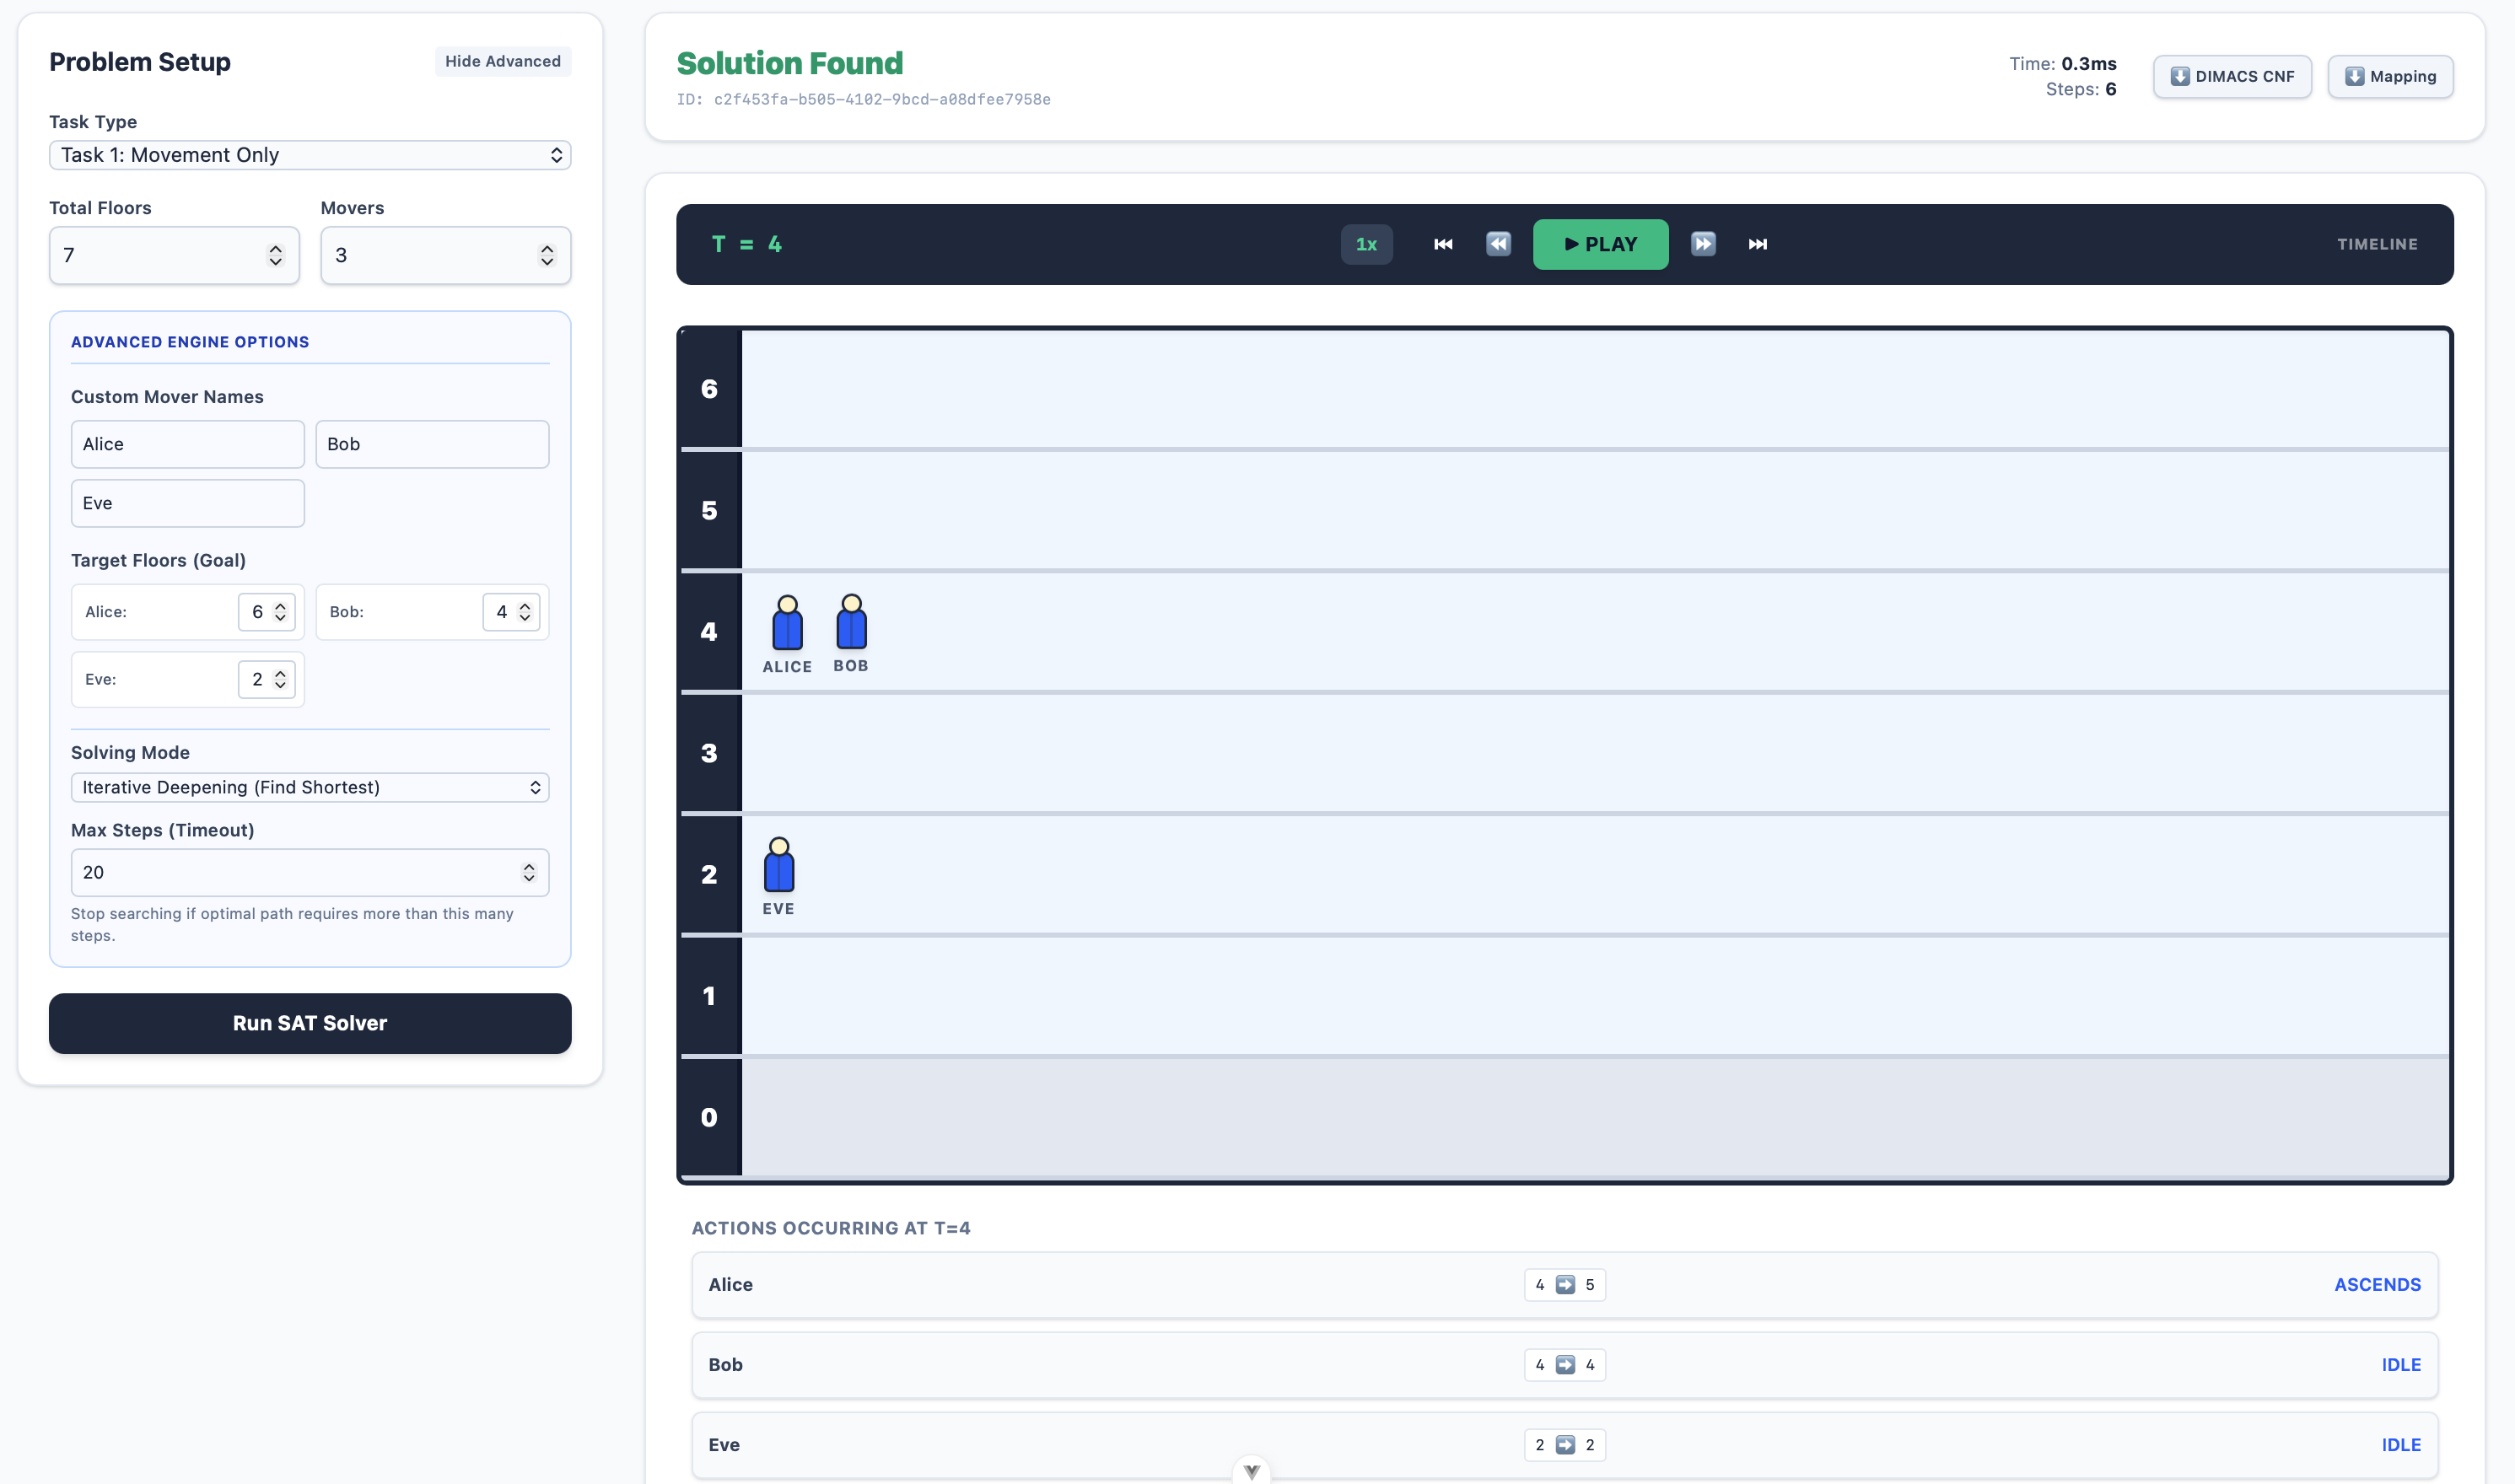
\includegraphics[width=0.95\textwidth]{img/task1-intermediate-state}
    \caption{Intermediate state of the Task 1 solution, where some movers have already reached their target floors.}
    \label{fig:task1-middle}
\end{figure}

\begin{figure}[H]
    \centering
    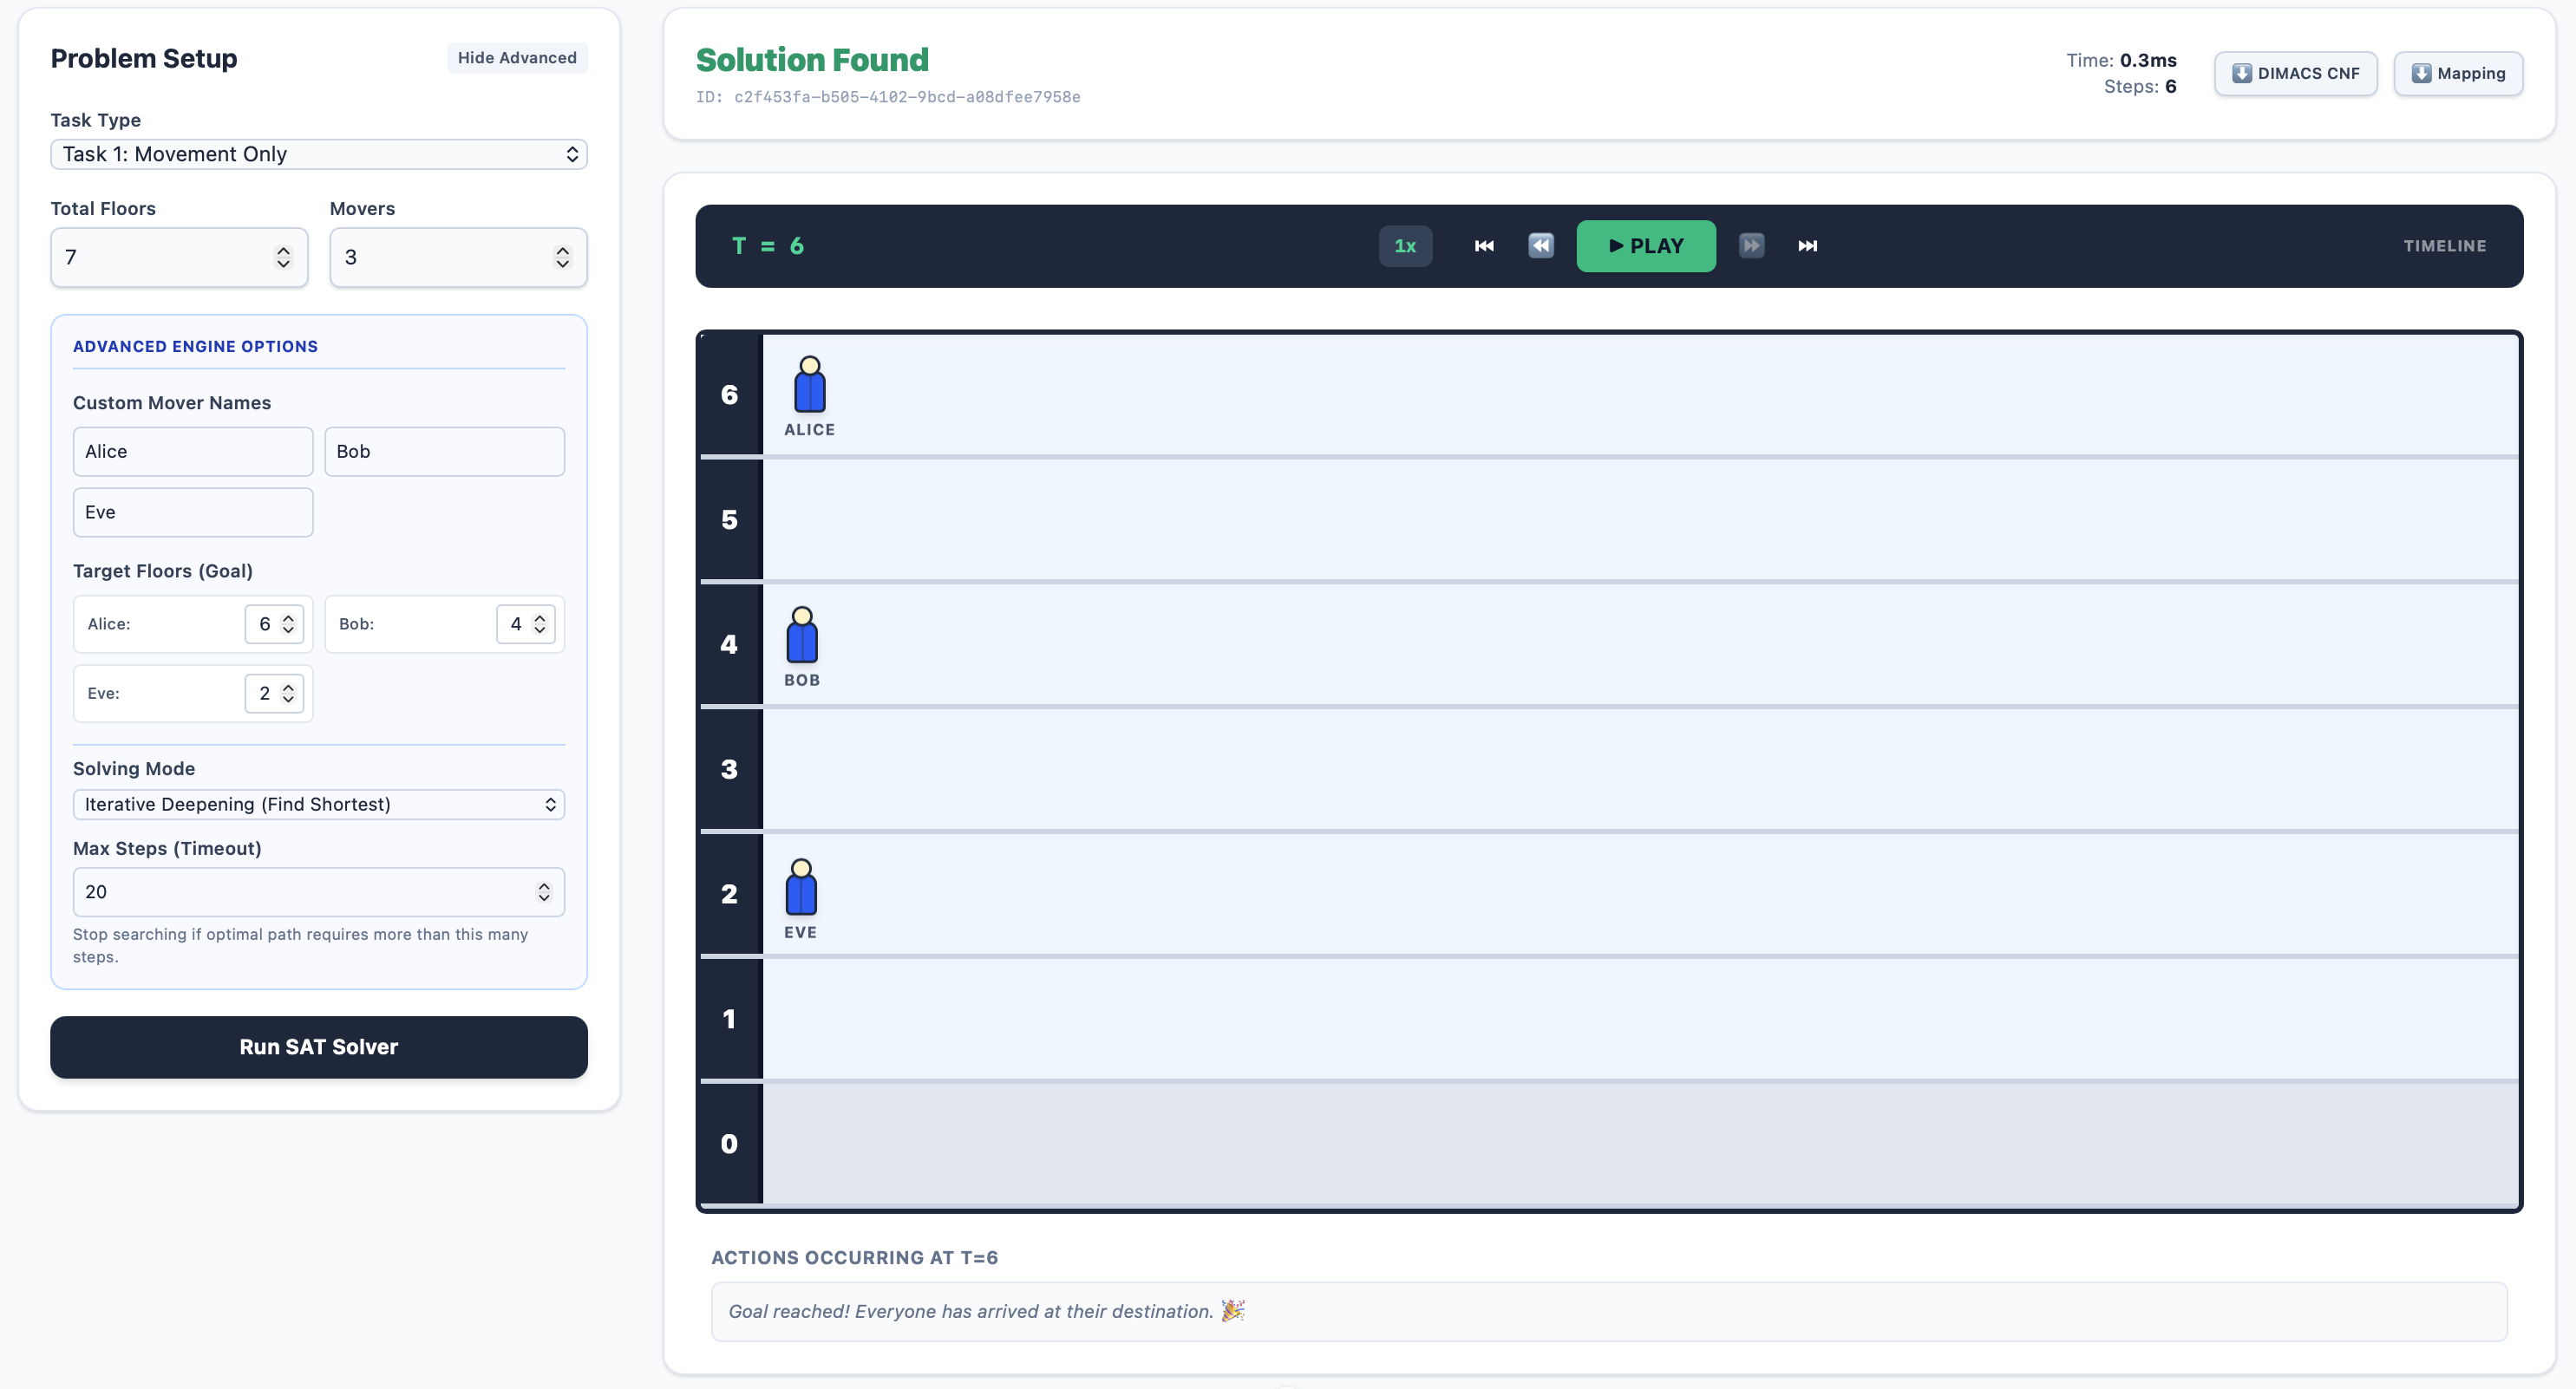
\includegraphics[width=0.95\textwidth]{img/task1-final-state}
    \caption{Final state of the Task 1 solution: Alice, Bob, and Eve are on their required target floors.}
    \label{fig:task1-final}
\end{figure}

\subsection{Case 2: Task 1 Unsatisfiable Within a Limited Horizon} \label{subsec:case-2:-task-1-unsatisfiable-within-a-limited-horizon}

The same Task 1 goal cannot be reached if the maximum allowed time horizon is too small.
For example, Alice must reach floor $6$ from floor $0$, so any solution requires at least six time steps.
If the search is stopped at $T_{\max}=4$, the solver correctly reports the instance as unsatisfiable within the given bound.

\begin{figure}[H]
    \centering
    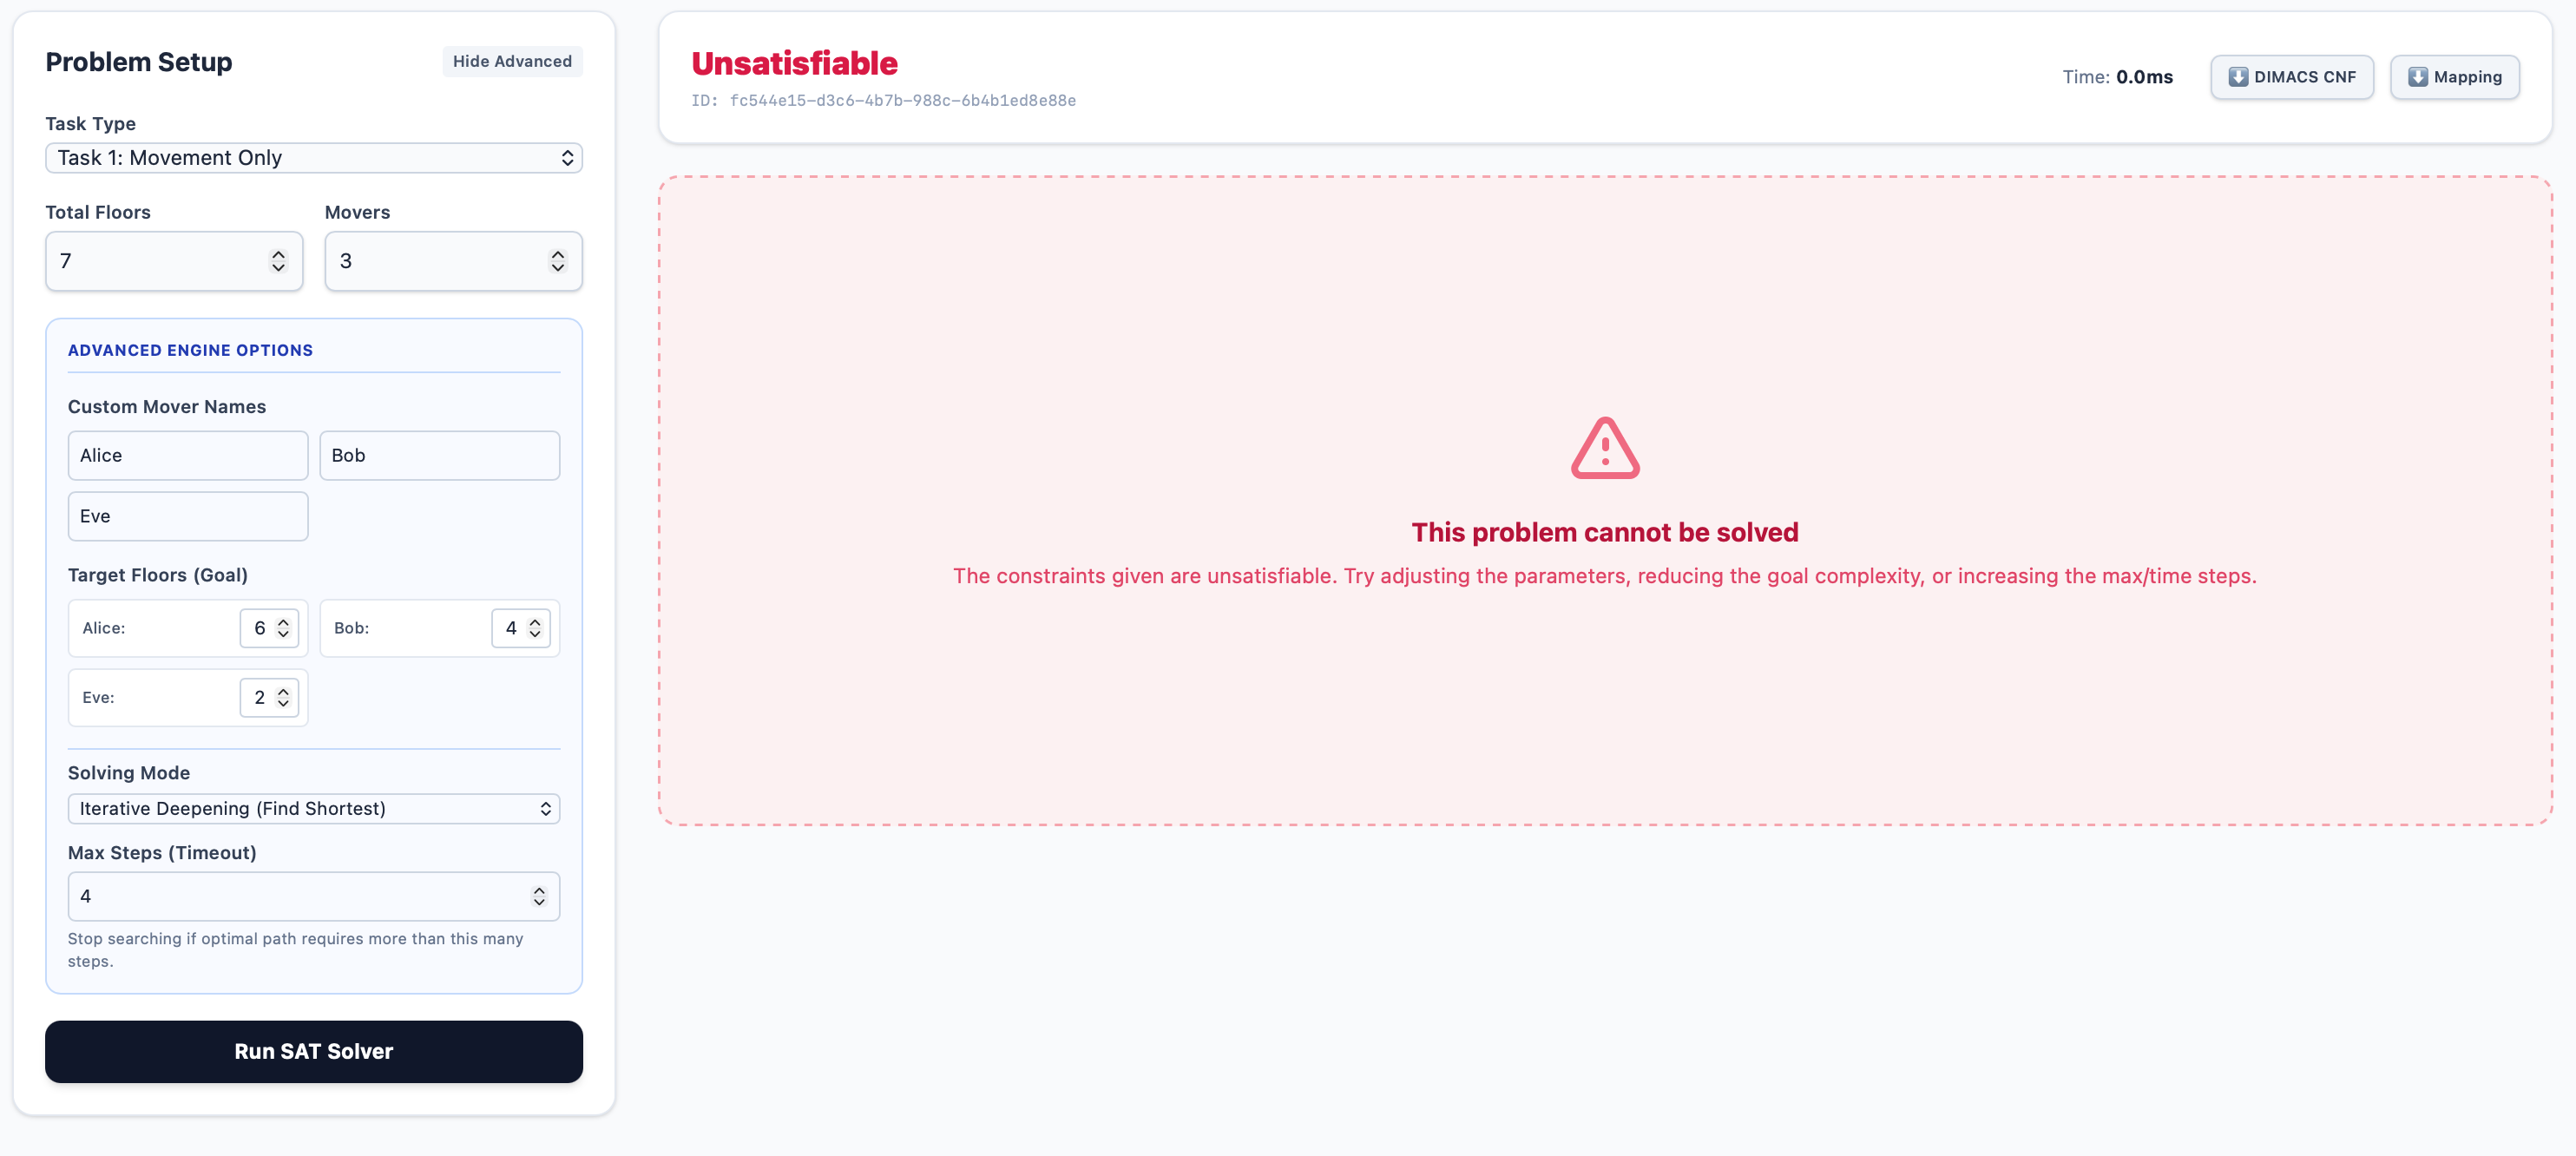
\includegraphics[width=0.95\textwidth]{img/task1-unsat-result}
    \caption{Task 1 unsatisfiable result when the maximum search horizon is too small to reach the target floors.}
    \label{fig:task1-unsat}
\end{figure}

\subsection{Case 3: Trivial Task 1 Goal} \label{subsec:case-3:-trivial-task-1-goal}

If the target floor is already floor $0$, then the initial state satisfies the goal.
The solver correctly returns a satisfiable result at $T=0$.

\subsection{Case 4: Task 2 with Three Items} \label{subsec:case-4:-task-2-with-three-items}

For the carrying task, a tested configuration uses three movers and three items:
\[
    \texttt{flowerpot}@2, \qquad
    \texttt{chair}@1, \qquad
    \texttt{table}@2.
\]

\noindent The solver finds a valid plan in four steps.
The final state places all movers and all items on floor $0$.

\subsection{Case 5: Task 2 Unsatisfiable Fixed-Horizon Instance} \label{subsec:case-5:-task-2-unsatisfiable-fixed-horizon-instance}

In this frontend test, the building has seven floors, two movers, and three items:
\[
    \texttt{Sofa}@3,\qquad
    \texttt{Desk}@4,\qquad
    \texttt{Chair}@6.
\]

\noindent The solver is executed in fixed-horizon mode with an exact time horizon of $T=10$.
The instance is reported as unsatisfiable, showing that the system correctly detects when no valid plan exists within the selected number of time steps.
This also confirms that the frontend properly displays bounded UNSAT results returned by the backend.


\begin{figure}[H]
    \centering
    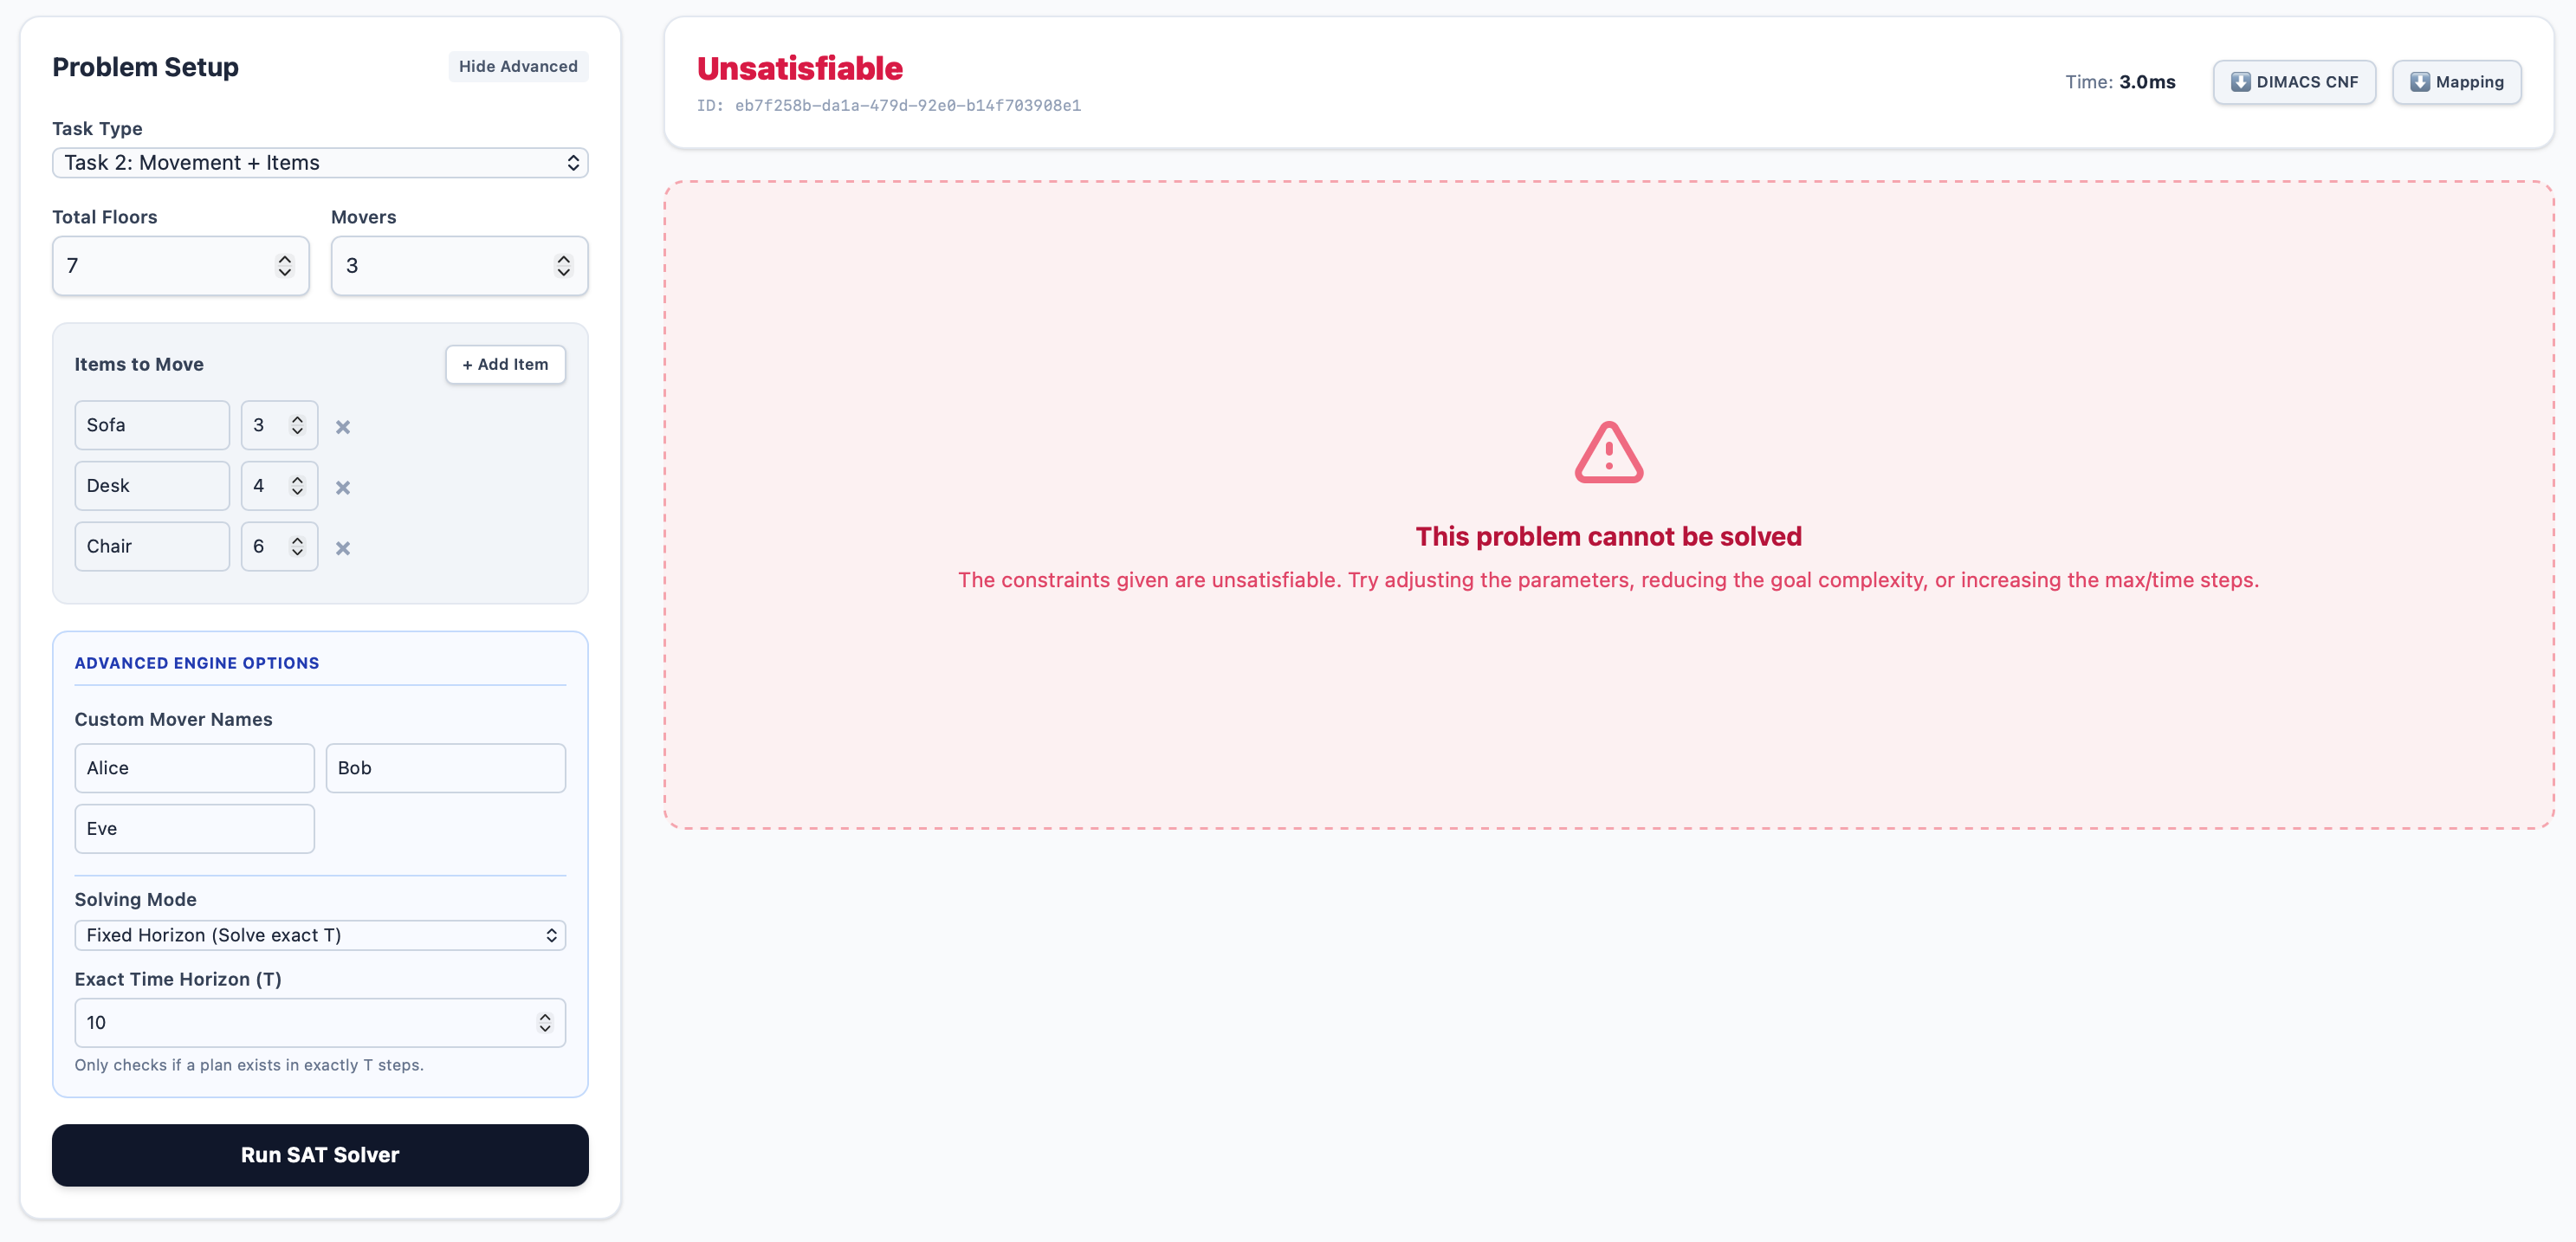
\includegraphics[width=0.95\textwidth]{img/task2-fixed-unsat}
    \caption{Frontend output for an unsatisfiable fixed-horizon Task 2 instance.}
    \label{fig:frontend-unsat}
\end{figure}

\subsection{Case 6: Full Example with Five Items} \label{subsec:case-6:-full-example-with-five-items}

The full example configuration contains:
\[
    \texttt{flowerpot}@2,\quad
    \texttt{chair}@1,\quad
    \texttt{table}@2,\quad
    \texttt{piano}@1,\quad
    \texttt{sofa}@2.
\]

\noindent The solver finds an optimal solution in six steps for this full configuration.
This confirms that the Task 2 encoding scales beyond the minimal three-item example.

\subsection{Case 7: Larger Custom Frontend Instance} \label{subsec:case-7:-larger-custom-frontend-instance}

A larger frontend example uses seven floors, three movers, and four items:
\[
    \texttt{Sofa}@3,\quad
    \texttt{Desk}@4,\quad
    \texttt{Chair}@6,\quad
    \texttt{Table}@1.
\]

\noindent The frontend visualization shows the movers and items progressing through the building until every object reaches floor $0$.
The solution is displayed with a timeline, action log, and final confirmation message.

\begin{figure}[H]
    \centering
    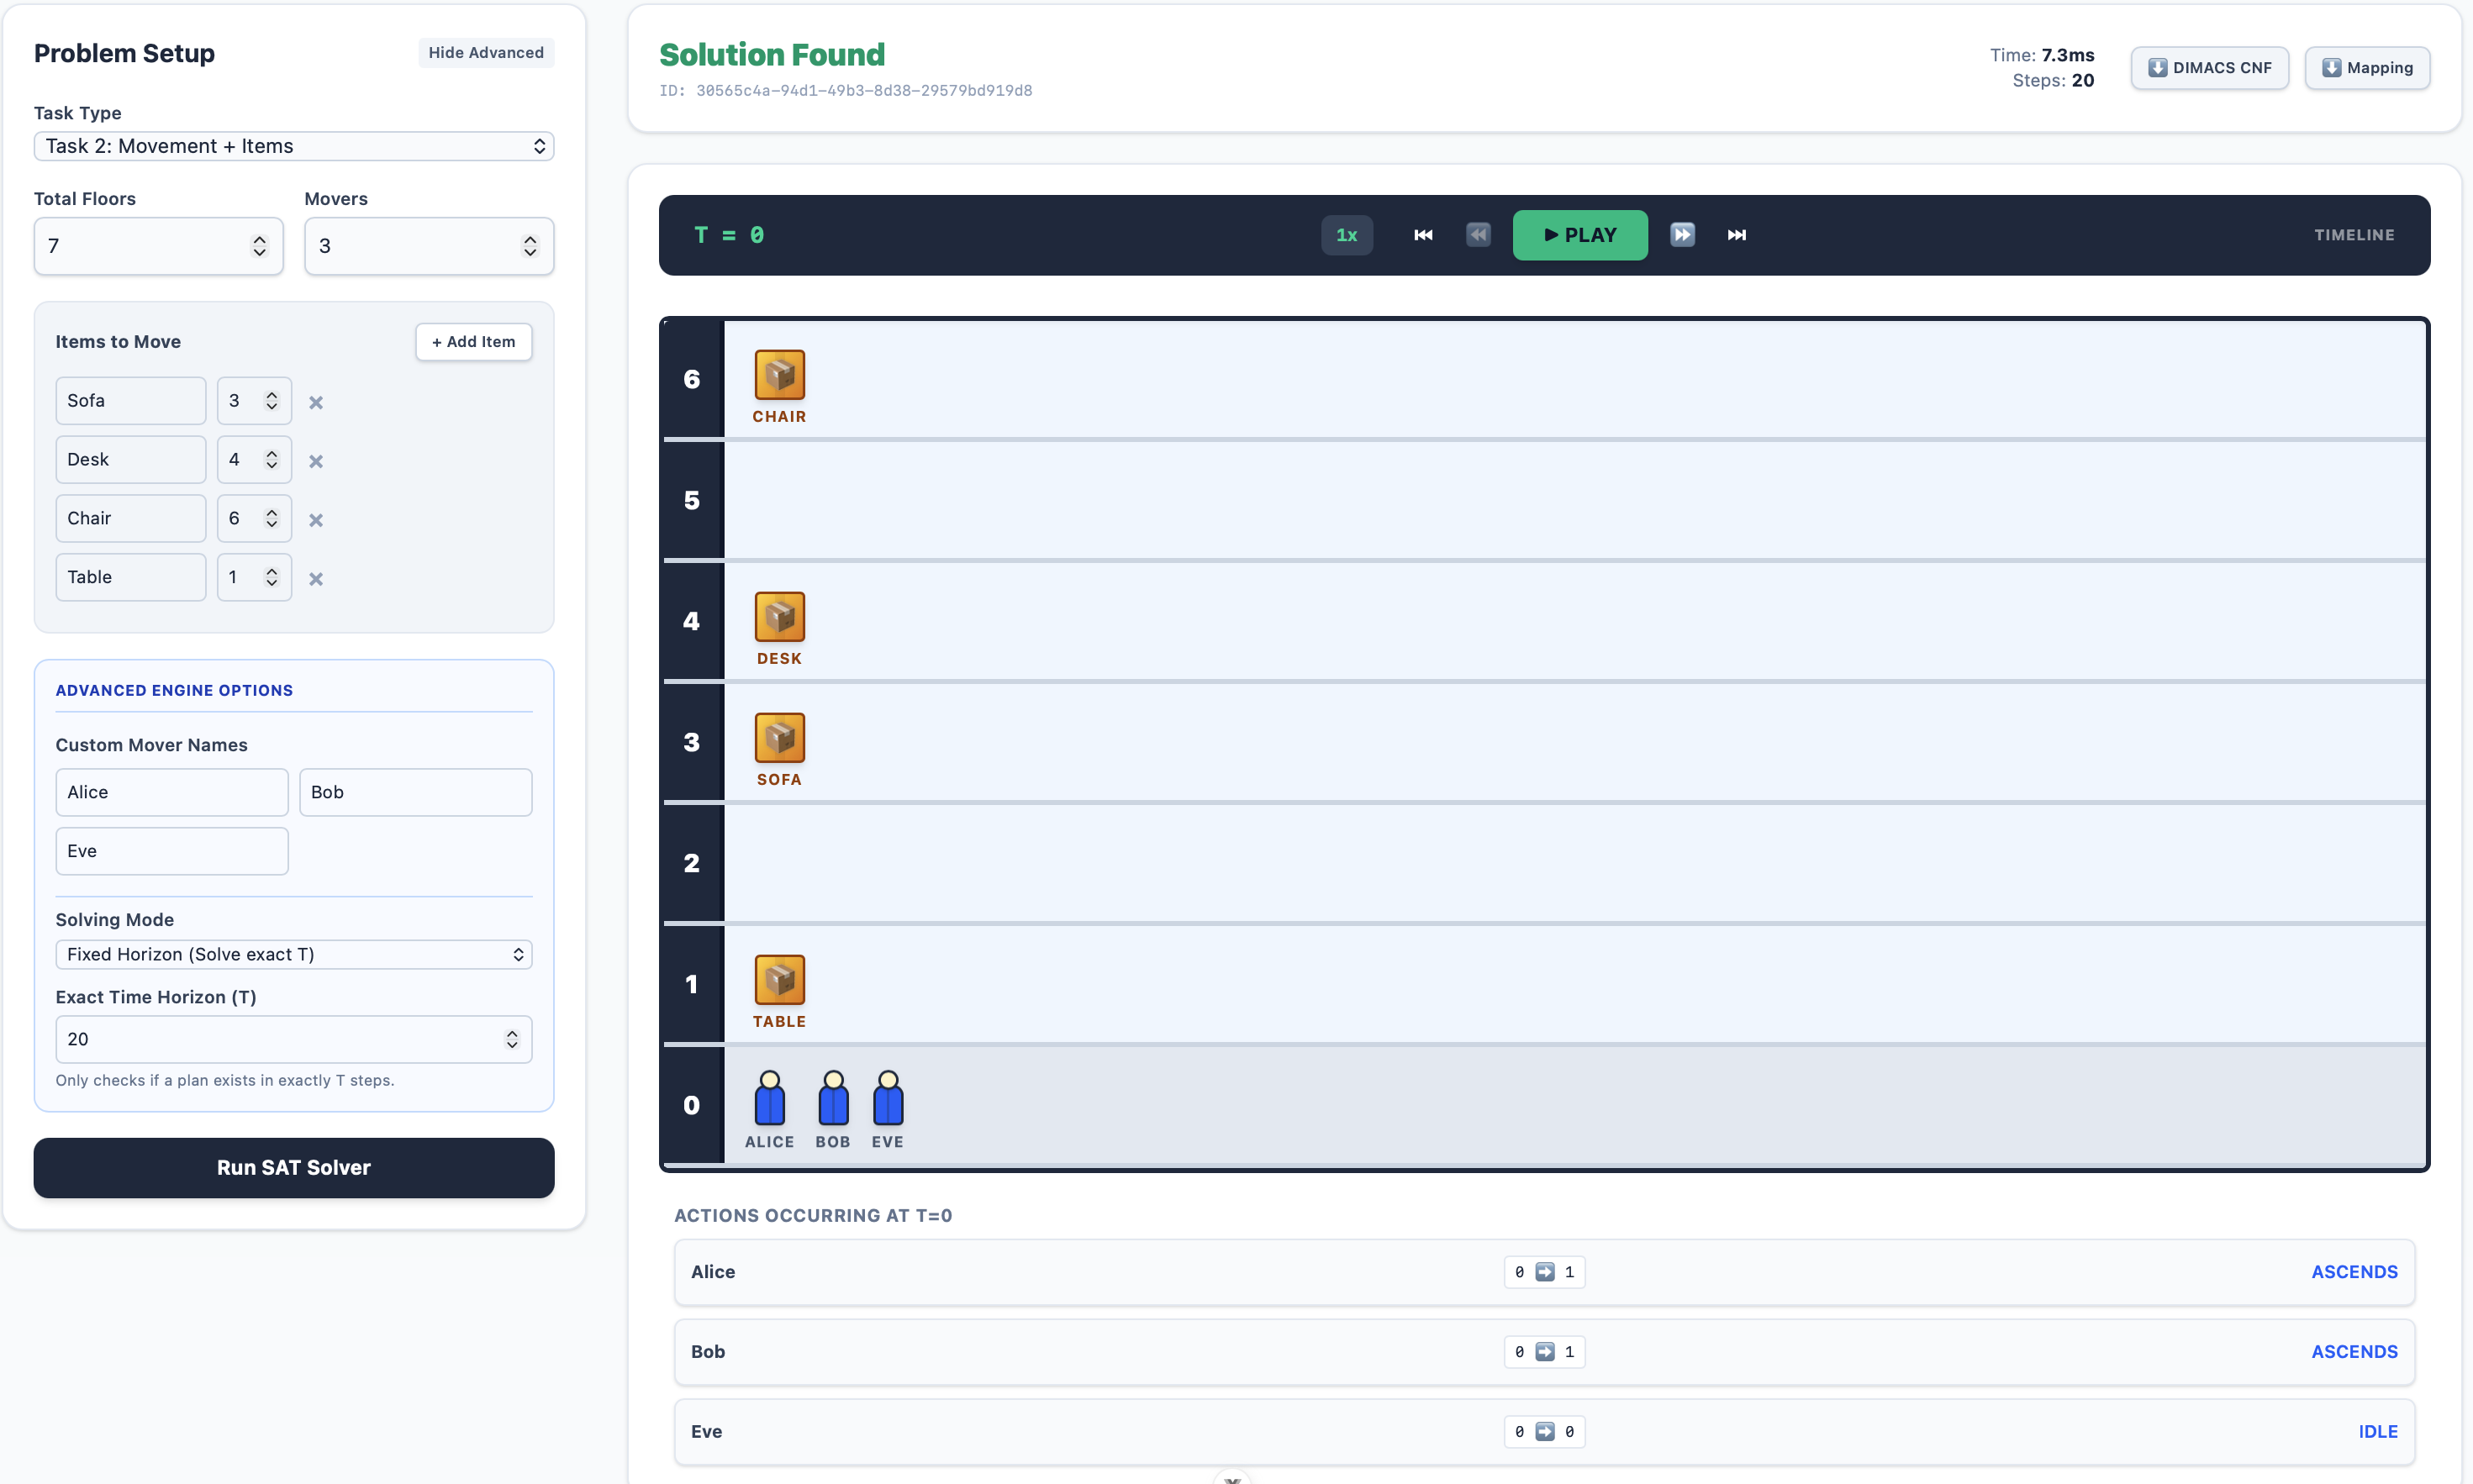
\includegraphics[width=0.95\textwidth]{img/task2-large-initial}
    \caption{Initial state of a larger Task 2 instance with seven floors, three movers, and four items.}
    \label{fig:large-instance-initial}
\end{figure}

\begin{figure}[H]
    \centering
    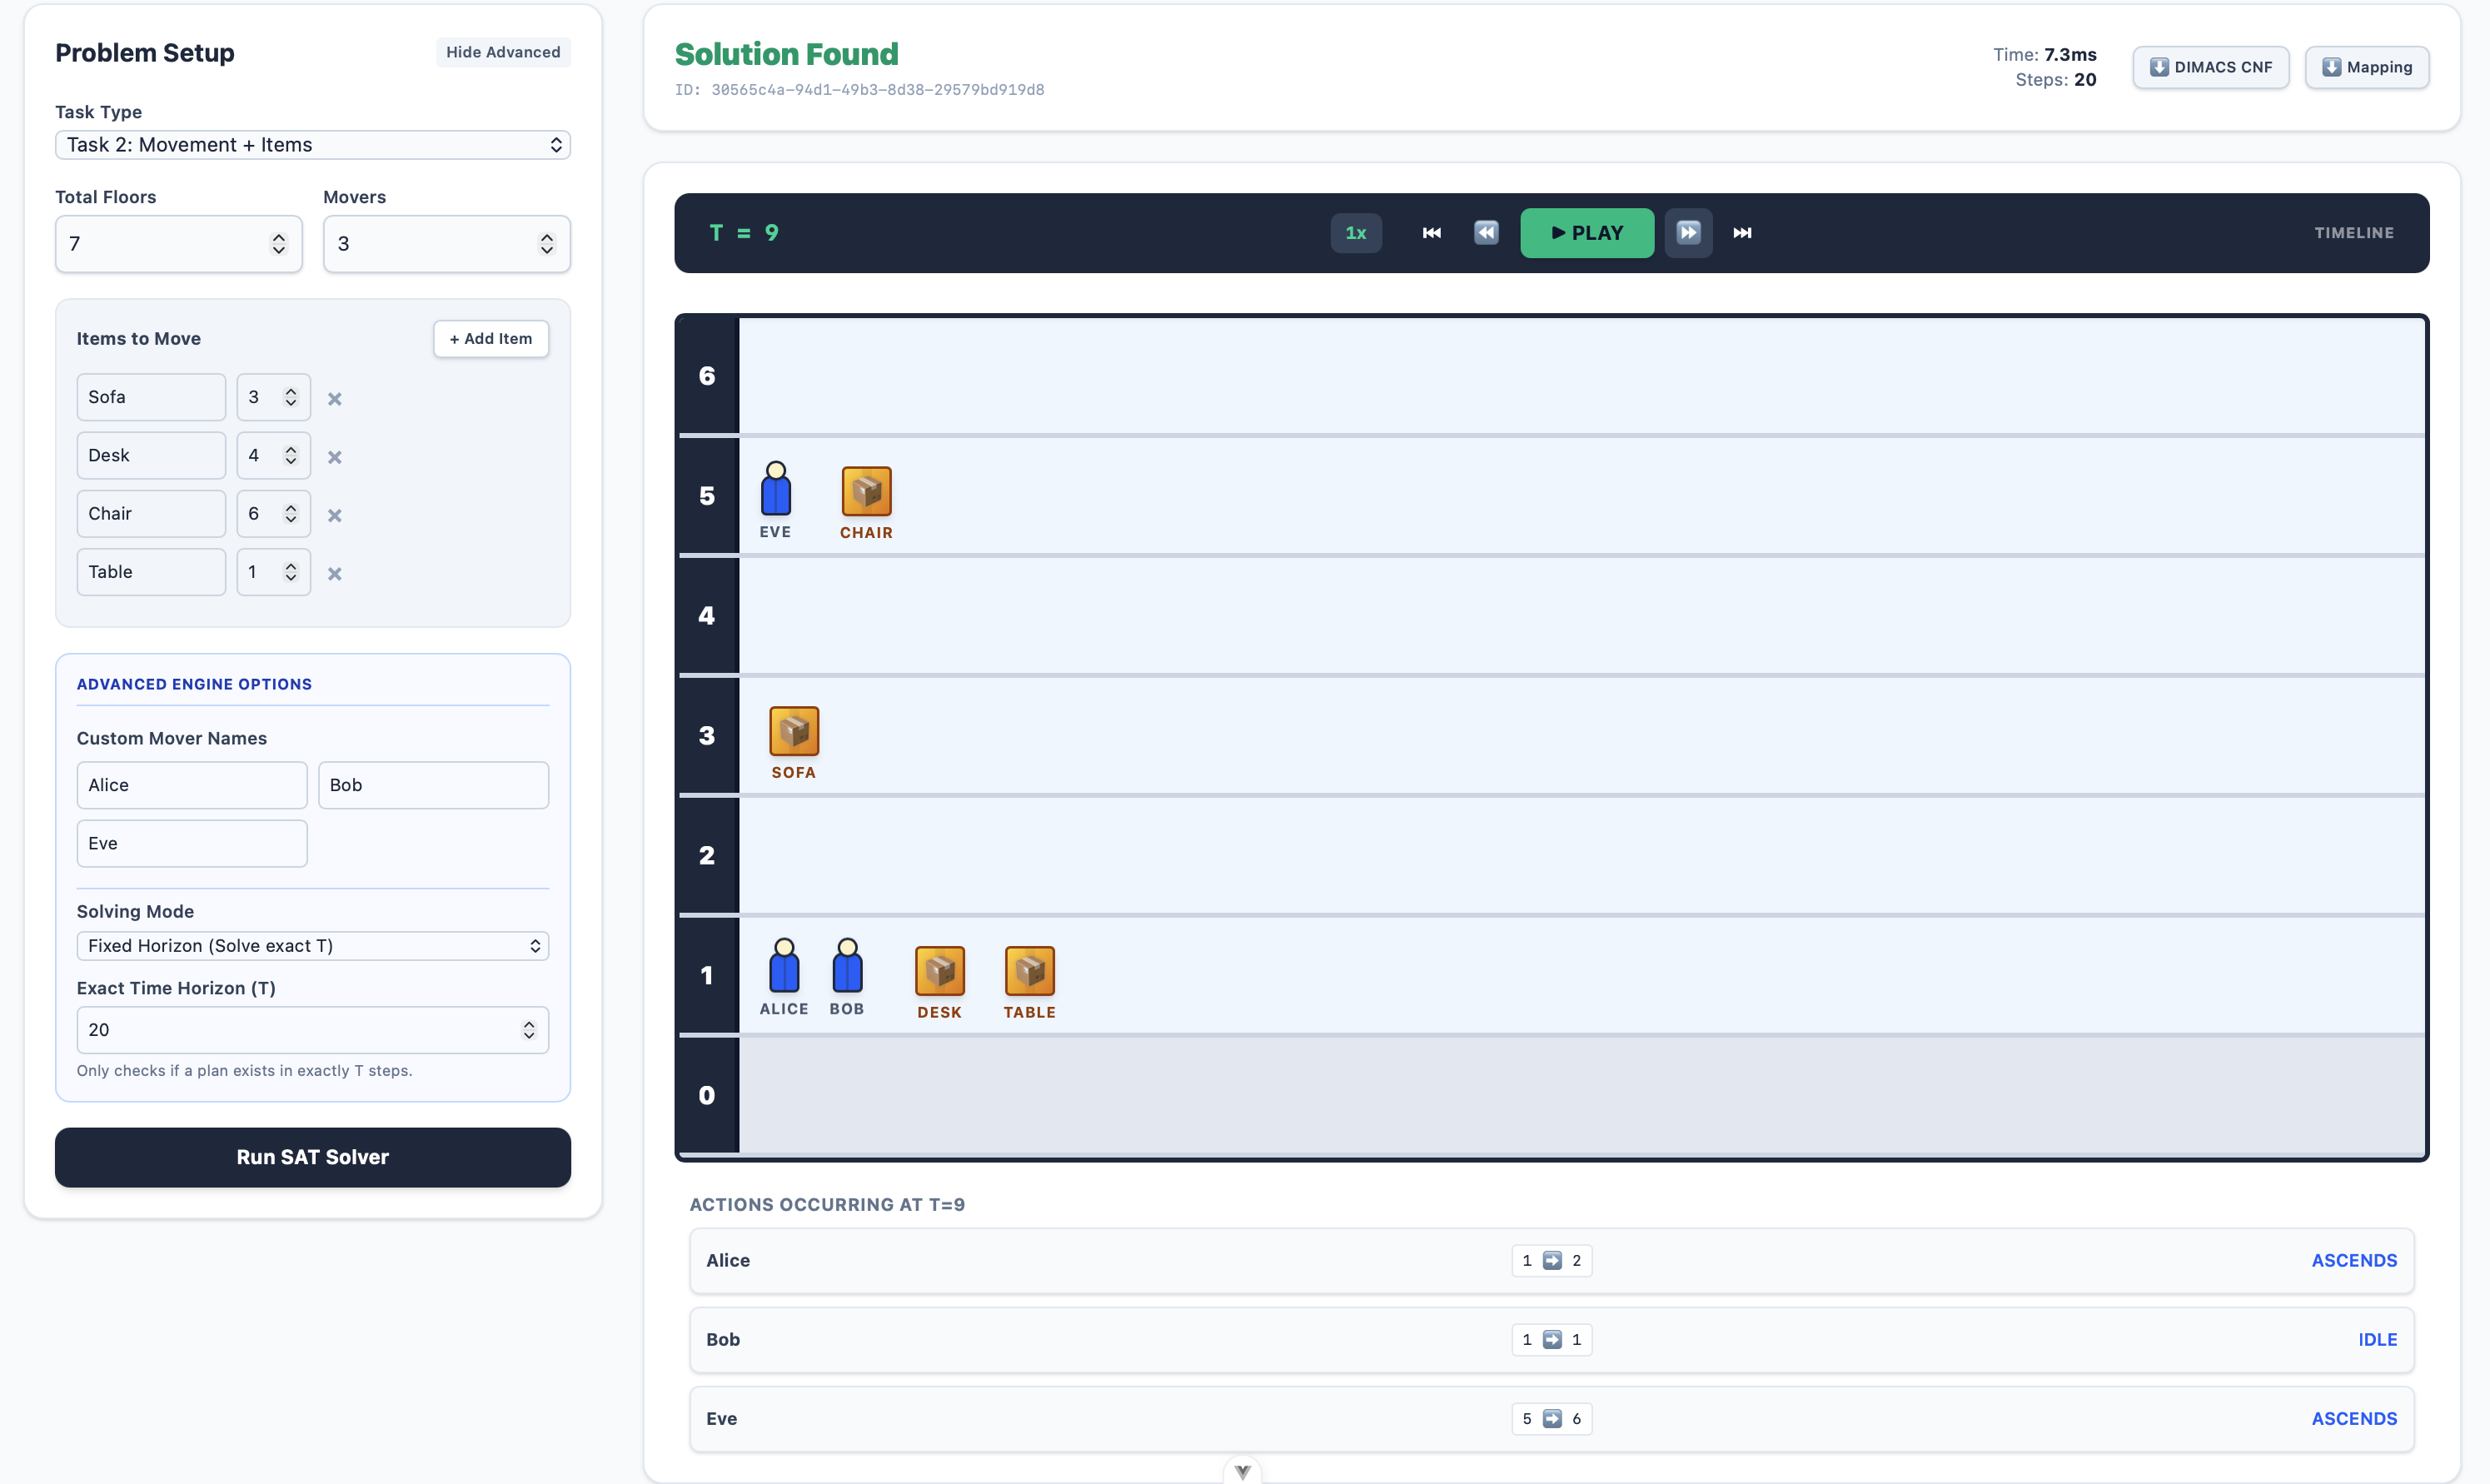
\includegraphics[width=0.95\textwidth]{img/task2-large-intermediate}
    \caption{Intermediate state of the larger instance, showing movers carrying items during the plan.}
    \label{fig:large-instance-middle}
\end{figure}

\begin{figure}[H]
    \centering
    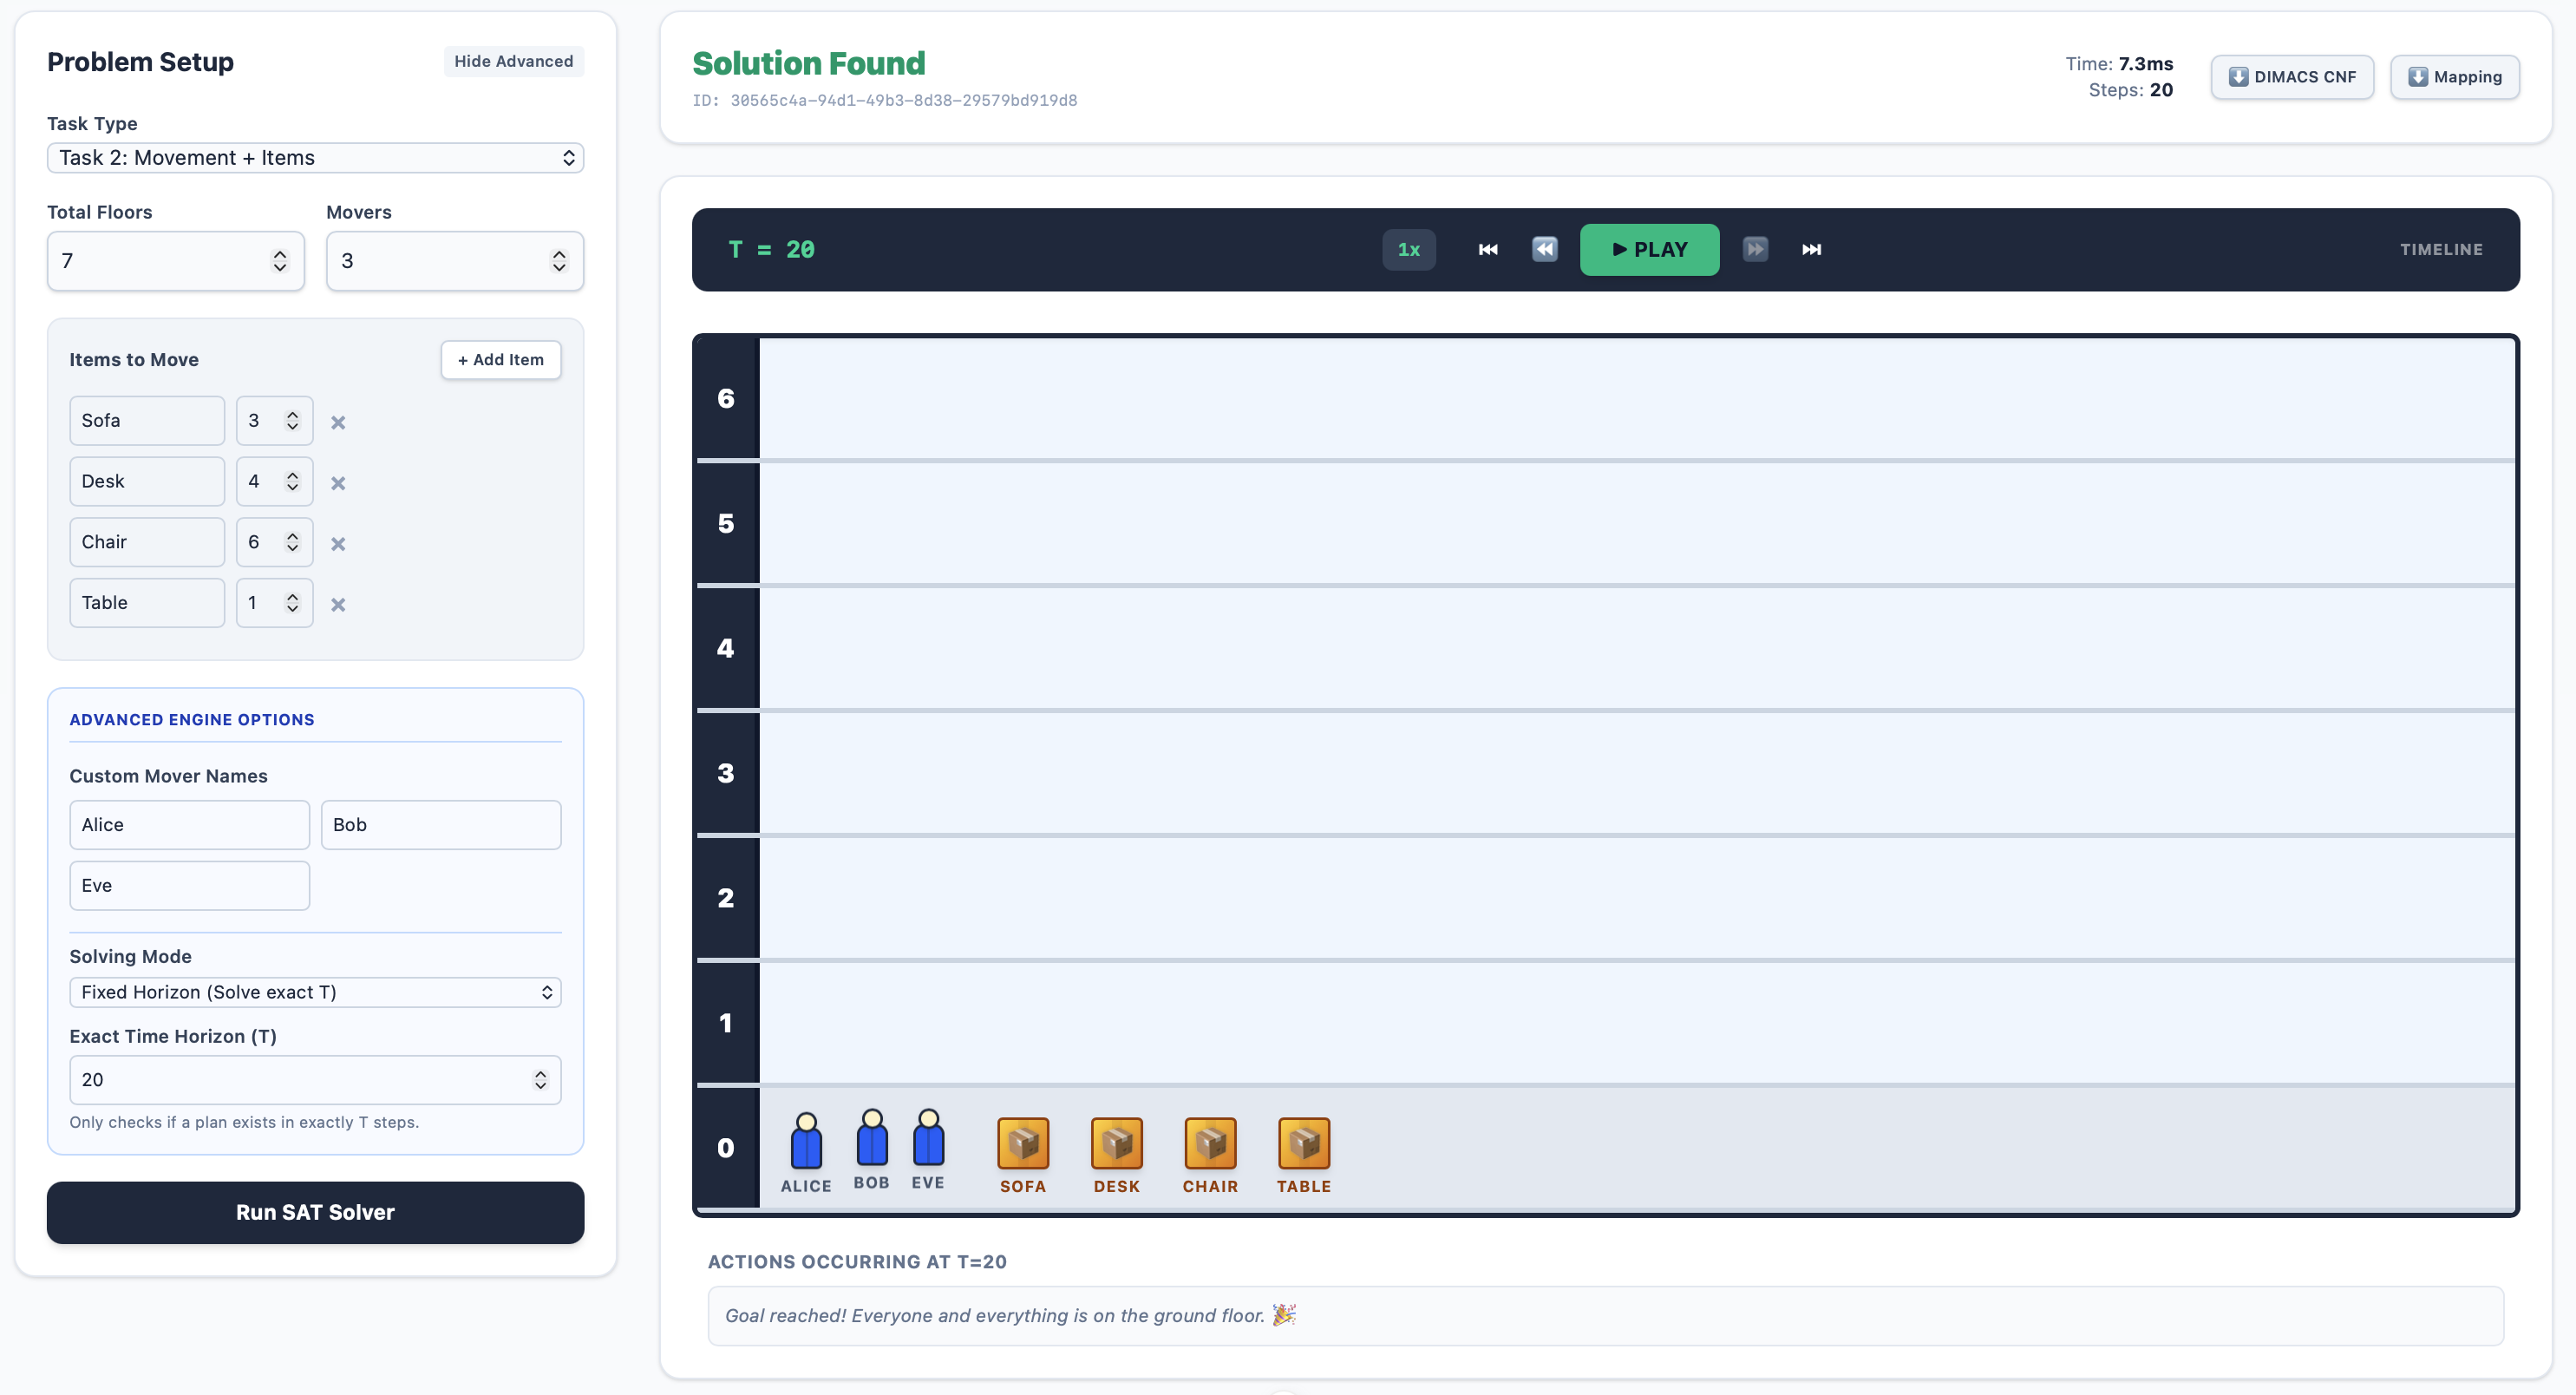
\includegraphics[width=0.95\textwidth]{img/task2-large-final}
    \caption{Final state of the larger instance, where all movers and items have reached the ground floor.}
    \label{fig:large-instance-final}
\end{figure}